\documentclass{standalone}
\usepackage{fontspec}
\setsansfont{DejaVuSans.ttf}[Path=./,Kerning=Off,Ligatures={TeXOff,NoCommon}]
\usepackage{tikz}
\begin{document}
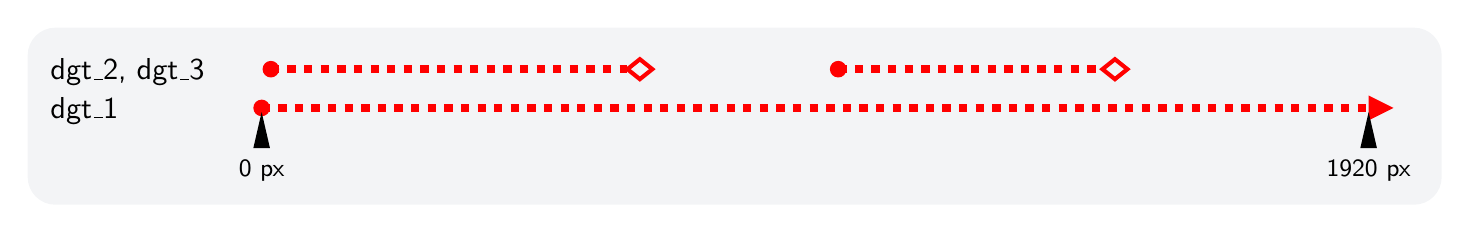
\begin{tikzpicture}[x=1pt,y=1pt,miter limit=4,font=\sffamily]
\definecolor{ts000000}{HTML}{000000}
\definecolor{tsF3F4F6}{HTML}{F3F4F6}
\definecolor{tsFF0000}{HTML}{FF0000}
\begin{scope}[shift={(16,16)}]
\path[rounded corners=10pt,fill=tsF3F4F6] (0,0) rectangle (510.948,63.9766);
\path[draw=tsFF0000,line width=3pt,dash pattern=on 3pt off 3pt] (84.5459,34.9766) -- (484.5459,34.9766);
\path[fill=tsFF0000] (84.5459,34.9766) circle[radius=3];
\path[fill=tsFF0000] (493.5459,34.9766) -- (484.5459,39.4766) -- (484.5459,30.4766) -- cycle;
\path[draw=tsFF0000,line width=3pt,dash pattern=on 3pt off 3pt] (87.8792,48.9766) -- (216.7126,48.9766);
\path[fill=tsFF0000] (87.8792,48.9766) circle[radius=3];
\path[draw=tsFF0000,line width=1.5pt] (216.7126,48.9766) -- (221.2126,52.5766) -- (225.7126,48.9766) -- (221.2126,45.3766) -- cycle;
\path[draw=tsFF0000,line width=3pt,dash pattern=on 3pt off 3pt] (292.8792,48.9766) -- (388.3792,48.9766);
\path[fill=tsFF0000] (292.8792,48.9766) circle[radius=3];
\path[draw=tsFF0000,line width=1.5pt] (388.3792,48.9766) -- (392.8792,52.5766) -- (397.3792,48.9766) -- (392.8792,45.3766) -- cycle;
\path[fill=ts000000] (84.5459,33.4766) -- (81.5459,20.4766) -- (87.5459,20.4766) -- cycle;
\path[fill=ts000000] (484.5459,33.4766) -- (481.5459,20.4766) -- (487.5459,20.4766) -- cycle;
\node[anchor=base west,inner sep=0,font=\sffamily\fontsize{11}{12.8047}\selectfont,text=ts000000] at (8,45.1685) {dgt\_2, dgt\_3};
\node[anchor=base west,inner sep=0,font=\sffamily\fontsize{11}{12.8047}\selectfont,text=ts000000] at (8,31.1685) {dgt\_1};
\node[anchor=base,inner sep=0,font=\sffamily\fontsize{9}{10.4766}\selectfont,text=ts000000] at (84.5459,10.1226) {0 px};
\node[anchor=base,inner sep=0,font=\sffamily\fontsize{9}{10.4766}\selectfont,text=ts000000] at (484.5459,10.1226) {1920 px};
\end{scope}
\end{tikzpicture}
\end{document}
